% datum?
\documentclass[thesis=B,czech,hidelinks]{FITthesis}[2019/03/06]

% my packages and stuff
\usepackage{todonotes}
\usepackage{xevlna}
% from https://tex.stackexchange.com/a/251025
\usepackage{relsize}
\usepackage{xspace}
\newcommand{\Rplus}{\protect\hspace{-.1em}\protect\raisebox{.35ex}{\smaller{\smaller\textbf{+}}}}
\newcommand{\Cpp}{\mbox{C\Rplus\Rplus}\xspace}
\usepackage[backend=biber,style=iso-numeric,sortlocale=cs_CZ,autolang=other,bibencoding=UTF8]{biblatex}
\usepackage[outputdir=build]{minted}
\renewcommand{\listingscaption}{Ukázka zdrojového kódu} %místo Listing ve výpisu bude Výpis kódu
\renewcommand{\listoflistingscaption}{Seznam ukázek zdrojového kódu} %místo List of Listings vypíšeme Seznam výpisů kódu
\counterwithin{listing}{chapter} %číslování prostředí listing v rámci kapitol

\addbibresource{mybibliographyfile.bib}

\hyphenation{NETCONF NETCONFu knihovnu knihovny}


\department{Katedra softwarového inženýrství}
\title{Nástroj pro konfiguraci a monitorování}
\authorGN{Václav}
\authorFN{Kubernát}
\authorWithDegrees{Václav Kubernát}
\author{Václav Kubernát}
\supervisor{Ing. Tomáš Čejka, Ph.D.}
% TODO: dopsat
\acknowledgements{Doplňte, máte-li komu a za co děkovat. V~opačném případě úplně odstraňte tento příkaz.}

\abstractCS{Tato práce se zabývá vytvořením interaktivní konzolové aplikace sloužící ke konfiguraci síťových zařízení pomocí protokolu \textit{NETCONF}. Tento program slouží jako alternativa k dostupným, méně intuitivním, řešením. Toho dosahuje přívětivým uživatelským rozhraním implementovaným pomocí kniho\-vny \textit{replxx}.

Řešení využívá generátorů parserů, které jsou definovány deklarativně, knihovnu \textit{libyang} pro manipulaci s modelovacím jazykem \textit{YANG} a \textit{libnetconf} pro komunikaci přes protokol \textit{NETCONF}.
}

\abstractEN{This thesis focuses on creating an interactive console application with the purpose of configuring network devices over the \textit{NETCONF} protocol. This program serves as an alternative to available, but less intuitive solutions. This is achieved mainly by creating a user-friendly interface implemented by the \textit{replxx} library.

The solution uses \textit{Boost Spirit X3} to create parsers defined declaratively, \textit{libyang} library for manipulating the \textit{YANG} modeling language, and \textit{\mbox{libnetconf}} for communication over \textit{NETCONF}.
}
\placeForDeclarationOfAuthenticity{V~Praze}
% TODO: zkontrolovat
\declarationOfAuthenticityOption{4} %volba Prohlášení (číslo 1-6)

\keywordsCS{netconf, yang, síťová konfigurace, konfigurace, cli, interaktivní cli, parsování}
\keywordsEN{netconf, yang, network configuration, configuration, cli, interactive cli, parsing}

\begin{document}

\begin{introduction}
Ke konfiguraci síťových zařízení existuje mnoho nástrojů. Pro klasického uživatele je nejlepší volba libovolného grafického rozhraní, ve kterém lze nastavit esenciální funkce jako například název nebo zabezpečení bezdrátové sítě. Pro síťové administrátory, kteří musí spravovat mnoho síťových zařízení najednou, je ovšem takové řešení nevhodné, protože jej nelze používat v různých skriptech apod. V těchto případech je tedy nutné použít konzolovou aplikaci. V této práci implementuji program, který umožní administrátorům jednoduše a intuitivně konfigurovat síťová zařízení.

Pokud chceme konfigurovat zařízení po síti, je třeba nejprve způsob komunikace se zařízeními standardizovat. \textit{NETCONF}\,\cite{rfcNetconf} byl vytvořen organizací IETF\footnote{Internet Engineering Task Force; organizace zabývající se vývojem internetových standardů} jako standard pro konfiguraci síťových zařízení. \textit{NETCONF} neřeší způsob reprezentace konfiguračních dat, a proto byl pro tyto potřeby vytvořen modelovací jazyk \textit{YANG}\,\cite{rfcYang}. Moje aplikace komunikuje s zařízeními právě pomocí těchto dvou standardů. Více o těchto standardech píši v teoretické části práce.

V návrhové části práce se věnuji tomu, jakým způsobem lze program používat a rozebírám syntaxi programu. Aplikace by měla být intuitivní, což znamená že by ji uživatel měl být schopný ovládat i bez detailní znalosti \textit{NETCONFu} nebo konkrétních modelů \textit{YANG}. Prostředky pro tuto \uv{intuitivnost} jsou zde popsány též.

Hlavním důvodem výběru této bakalářské práce je především využití znalostí ohledně teorie formálních jazyků a gramatik. Aplikace využívá generátoru parserů \textit{Boost Spirit X3}\,\cite{boost:spirit} k realizaci syntaxe, pomocí které je program ovládán. O knihovně \textit{Spirit} a dalších prostředcích, které moje aplikace využívá, pojednává implementační část práce.
\end{introduction}

\chapter{Teoretická část}
V rámci práce se věnuji různým klíčovým technologiím a pojmům. V této kapitole vysvětluji použité standardy a teorii formálních jazyků, která mi pomáhá s vytvářením parserů.


\section{YANG}
\textit{YANG} je jazyk sloužící k modelování konfigurace. Pomocí různých zabudovaných konstruktů lze vybudovat konfigurační strom, který logicky sdružuje různé druhy konfigurace, definuje, kde lze jakou hodnotu nastavit, jaké mají hodnoty datové typy apod. Kromě konfigurace podporuje \textit{YANG} i definování různých procedur. Kódování dat funguje pomocí XML\footnote{Extensible Markup Language; značkovací jazyk sloužící především k ukládání a přenosu dat}\@.

\textit{YANG} definuje konfigurační modely pomocí tzv. \textit{modulů}. Modul je základní složkou konfigurace a vše ostatní se definuje v něm. \textit{YANG} podporuje mnoho prostředků, kterými lze konfiguraci definovat. V ukázce~\ref{yang:ukazka} lze vidět syntaxi \textit{YANGu} s některými základními definicemi\footnote{slovo \uv{definice} používám jako náhradu anglického slova \uv{statement}}.

Definice lze dělit dle dvou kritérií:

\begin{enumerate}
    \item Dle množnosti přidávat vnořené definice
        \begin{itemize}
            \item Definice, které umožňují vnořovat definice lze poznat podle složených závorek
            \item Definice, které neumožňují vnořovat definice končí středníkem
        \end{itemize}
    \item Dle toho, jestli vytváří nový uzel
        \begin{itemize}
            \item Definice, které vytváří nový uzel mají syntaxi \texttt{<typ~uzlu>~<název~uzlu}. Název musí být unikátní.
            \item Definice, které nevytváří nový uzel.
        \end{itemize}
\end{enumerate}

Dále popisuji, co znamenají definice z ukázky~\ref{yang:ukazka}.\footnote{ačkoli lze jednotlivé názvy přeložit do češtiny, budu používat anglická označení, aby nedošlo k záměně některých termínů (list -- leaf, list -- seznam)}

\begin{listing}
\begin{verbatim}
module example-schema {
    prefix ex;
    namespace "http://example.com";

    container ip_adress {
        leaf ip {
            type string;
        }
        leaf mask {
            type string;
        }
    }
    leaf leafInt {
        type int32;
    }
    list aList {
       key "name";
       leaf name {
         type string;
       }
    }
}
\end{verbatim}
\caption{Ukázkový \textit{YANG} modul}\label{yang:ukazka}
\end{listing}
\subsection{\texttt{module}}
Kořen konfiguračního stromu je \texttt{module}. Označuje jednotný celek a ostatní je definováno v něm. V ukázce~\ref{yang:ukazka} jsou vidět jeho požadované definice. Jedna z nich je \texttt{namespace}, což je konstrukt jazyka XML, a druhá je \texttt{prefix}, která umožňuje nastavit zkratku, kterou můžeme následovně použít při odkazování na tento modul.

\subsection{\texttt{leaf}}
\texttt{leaf} slouží k nastavování samotných hodnot konfigurace. Jeho jedinou povinnou vnořenou definicí je \texttt{type}, která určuje, jaký datový typ bude hodnota mít. Datových typů existuje mnoho. Od základních jako řetězec nebo celé číslo, až po složitější jako například leafref, jehož hodnota (a datový typ) závisí na hodnotě jiného \texttt{leafu}.
\subsection{\texttt{container}}
\texttt{container} je základní prostředek pro sdružování konfigurace do logických celků. V ukázce~\ref{yang:ukazka} můžeme vidět sdružení \texttt{leafů} s názvy \texttt{ip} a \texttt{mask} pod jeden logický celek \texttt{ip-address}. \texttt{Container} sám od sebe nenese žádným význam pokud ovšem neobsahuje definici \texttt{presence}. V tomto případě se jedná o \texttt{presence container} a jeho přítomnost poté nese význam.
\subsection{\texttt{list}}
\texttt{list} slouží podobně jako \texttt{container} ke sdružování dat. Rozdíl mezi nimi je ten, že \texttt{list} může existovat ve více instancích najednou (\texttt{container} jen v jedné). Tyto instance se rozlišují pomocí klíče, což je hodnota nějakého \texttt{leafu} uvnitř daného \texttt{listu}. Klíč se definuje pomocí definice \texttt{key} a může jich být i více (instance je poté definovaná pomocí obou klíčů zároveň).


\section{NETCONF}
\textit{NETCONF} je protokol vytvořený organizací IETF sloužící ke vzdálené úpravě konfigurace síťových zařízení. Kromě konfigurace lze pomocí \textit{NETCONFu} implementovat zjišťování různých informací o stavu zařízení nebo se přihlašovat k různým oznámením. Je založen na architektuře server-klient (tato práce se zabývá implementací klientské části). Při komunikaci přes \textit{NETCONF} zasílá klient serveru zprávy prostřednictvím XML-RPC.\footnote{protokol založený na značkovacím jazyku XML, umožňující jednoduché volání vzdálených procedur} Samotné zasílání zpráv na nižší úrovni probíhá přes protokol TLS nebo SSH -- protokoly umožňující vytváření šifrovaých spojení po síti.

Při zahájení komunikace si server i klient vymění \uv{hello} zprávu, ve které deklarují podporované \textit{capabilities} -- definice operací, které dané zařízení podporuje. Základní \textit{NETCONF} podporuje několik typů operací. Dále jsou popsány ty, kterými se zabývám.

\subsection{\texttt{<get>}}
Tato zpráva slouží k získání libovolné části konfiguračního stromu. To může být konfigurace anebo stavová informace. Server odpovídá zprávou \texttt{<rpc-reply>} s požadovanými daty nebo zprávou \texttt{<rpc-error>} při chybě.

\subsection{\texttt{<get-config>}}
Tato zpráva se podobá zprávě \texttt{<get>}. Rozdíl je v tom, že pomocí \texttt{<get-config>} lze získat konfiguraci z různých druhů datových úložišť. \textit{NETCONF} podporuje datová úložiště trojího druhu:
\begin{description}
    \item[running]{aktuální platná konfigurace}
    \item[startup]{startovní konfigurace, která se aplikuje při spuštění zařízení}
    \item[candidate]{pracovní konfigurace, která může být zkopírována do running konfigurace}
\end{description}

\subsection{\texttt{<edit-config>}}
\texttt{<edit-config>} slouží k úpravě konfiguračního stromu na serveru. Klient zašle úpravy ve formě podstromu a vybere, jestli chce tuto část sloučit s aktuálním podstromem, smazat, přepsat apod.

\section{Teorie formálních jazyků a gramatiky}
V této práci se také velmi často zabývám gramatikami z teorie formálních jazyků. Formální jazyk je množina řetězců vytvořených pomocí nějaké abecedy. Jazykem může být i syntaxe příkazů libolovného programu, což je i případ aplikace, kterou implementuji. Tyto formální jazyky lze mimo jiné zapsat pomocí formálních gramatik -- předpisů, které určují, jakým způsobem  lze vytvořit slova patřící do daného jazyka.\,\cite{formal-languages}

Formálně, gramatika je čtveřice $(N, \Sigma, P, S)$, kde $N$ je množina neterminálů\footnote{znaky, které jsou pouze náhradami za reálné znaky z abededy}, $\Sigma$ je množina literálů\footnote{znaků abecedy, z které se skládájí slova jazyka}, $P$ je množina pravidel, podle kterých se vytváří slova a $S$ je počáteční neterminál, od kterého vytváření slov začíná. Při tvorbě slov se nejprve vezme počáteční neterminál. Pomocí pravidel se poté neterminál přepisuje na další neterminály a literály. Toto se opakuje dokud se všechny neterminály nepřepíšou na literály.

Jeden ze způsobů, jakým zapisovat pravidla gramatiky, je pomocí \textit{EBNF}.\footnote{Extended Backus--Naur form; rozvinutá Backusova--Naurova forma} Tento způsob zápisu byl vytvořen za účelem vytvoření prostředku, kterým by bylo možné zapsat syntaxi jakéhokoliv programovacího jazyka.\,\cite{ebnf-cmu} Formou \textit{EBNF} se v této práci zabývám především kvůli její podobnosti se zápisem gramatik v knihovně \textit{Boost Spirit X3}. Pravidla zapsaná v \textit{EBNF} lze vidět na následující ukázce (počáteční pravidlo je pravidlo \texttt{start}):
\clearpage
\begin{verbatim}
start = 'a' , { letter };
letter = "a" | "b" | "c" | "d" | "e" | "f" | "g"
       | "h" | "i" | "j" | "k" | "l" | "m" | "n"
       | "o" | "p" | "q" | "r" | "s" | "t" | "u"
       | "v" | "w" | "x" | "y" | "z" ;
\end{verbatim}
Syntaxe \verb¨<nazev> =¨ definuje pravidla. Literály jsou uváděny pomocí znaků uvnitř uvozovek. Znak svislá čára \texttt{|} značí alternativu, což znamená, že neterminál lze nahradit za jakýkoliv symbol oddělený touto čarou. Neterminál \texttt{letter} tedy umožňuje nahrazení za jakýkoliv znak abecedy. Tento neterminál je použit v pravidle \texttt{start}. Čárka (\texttt{,}) slouží k zřetězení (\uv{slepení}) dvou jiných řetězců a složené závorky (\texttt{\{} a \texttt{\}}) znamenají, že cokoli uvnitř lze opakovat v libovolném počtu (i nula krát). Pravidla se oddělují středníkem (\texttt{;}). Gramatika z ukázky odpovídá jazyku, jenž obsahuje slova, která začínají písmenem \uv{a} a poté následuje libovolný počet písmen abecedy.



\chapter{Návrh}
V této kapitole nejprve popisuji existující programy, které implementují klientskou část protokolu \textit{NETCONF} a zdůvodňuji, proč je třeba vytvořit aplikaci novou. Dále se zabývám tím, jak program vypadá, syntaxí uživatelského vsttupu, a dalšími konstrukty, které se v mém programu vyskytují. Popisuji zde, jakým způsobem se uživatel orientuje ve stromech modelů \textit{YANG} a nakonec popisuji veškeré příkazy, které jsou v programu obsaženy.

\section{Existující relevantní práce}\label{existing}
V této kapitole popisuji požadavky aplikace a zdůvodňuji nutnost vytvoření nového nástroje pro vzdálenou konfiguraci.

V tento moment existuje několik programů implementující klientskou část \textit{NETCONFu}. Jeden z nich je \textit{Netopeer2-cli}\,\cite{netopeer} implementovaný v jazyce C. Pro komunikaci přes \textit{NETCONF} využívá knihovnu \textit{libnetconf}\,\cite{libnetconf}. Výhodou je, že podporuje takřka veškeré konstrukty \textit{NETCONFu} včetně připojení přes TLS a SSH\@. Dalším programem je \textit{netconf-console}\,\cite{netconf-console}. Ta je implementována v programovacím jazyku Python s pomocí knihovny \textit{ncclient}\,\cite{ncclient}.

Nevýhoda obou těchto aplikací je, že přestože jsou obě schopny konfigurace zařízení, jejich rozhraní není přívětivé, jelikož pohlíží na věc z hlediska protokolu \textit{NETCONF} a ne z hlediska toho, co chce uživatel konfigurovat. To v praxi znamená, že uživatel musí znát podrobně různé operace jako například \texttt{<get-config>} apod.


\section{Koncepce programu}
Program, který implementuji, je koncipován jako interaktivní konzolová aplikace. Silnou stránkou konzolových aplikací je možnost použití ve skriptech\footnote{skripty jsou jednoduché programy, používané k definování scénářů, například \uv{nastav údaj \texttt{x} zařízení \texttt{y} na hodnotu \texttt{z}}}. Uživatel může aplikaci použít interaktivně, napojením terminálu na vstup programu a manuálním zadáváním příkazů, ale také dávkově, uložením příkazů do souboru a vložením tohotu souboru na vstup programu.

\section{Adresování stromu}
Aby se mohl uživatel odkazovat na jednotlivé uzly ve stromu, je nejprve třeba vytvořit textový zápis, který jednoznačně určuje lokaci jednoho uzlu. K tomuto jsem zvolil podobný způsob jako adresování souborů a adresářů v souborovém systému. Cesta k uzlu je určena výčtem názvů všech uzlů, které je dělí od modulu. Vzhledem k tomu, že modulů může být mnoho, je třeba určit \uv{kontextový} modul, tedy modul, v kterým se nachází první uzel cesty. Toho lze docílit připsáním názvu modulu a dvojtečky před první uzel cesty. Cesta k uzlu \texttt{bar} (nacházející se v uzlu \texttt{foo}) v modulu \texttt{example-schema} z ukázky~\ref{yang:adresace} bude vypadat takto: \texttt{example-schema:foo/bar}. Může se stát, že v nějaké části cesty, budeme chtít \uv{kontextový} modul změnit, a proto je možné název modulu a dvojtečku připsat ke každému uzlu.\footnote{cesta k \texttt{bar} by tedy mohla vypadat i takto: \texttt{example-schema:foo/example-schema:bar}}

\begin{listing}
\begin{verbatim}
module example-schema {
    prefix ex;
    namespace "http://example.com";

    container foo {
        leaf bar {
            type string;
        }
    }
}
\end{verbatim}
\caption{\textit{YANG} modul s uzly typu \texttt{container} a \texttt{leaf}}\label{yang:adresace}
\end{listing}

Adresovat lze dvěma způsoby: relativními cestami a absolutními cestami. Relativní cesty se vztahují ke kontextu, v kterém uživatel je. Pokud je aktuální kontext uzel \texttt{example-schema:foo} a chceme adresovat uzel \texttt{bar}, není již třeba v cestě uzel \texttt{foo} zahrnovat a ani není třeba specifikovat kontextový modul. Na druhou stranu, absolutní cesty nedbají na kontext a chovají se, jako kdyby žádný kontext neexistoval. Absolutní cesty se zapisují s lomítkem (\texttt{/}) na začátku.

Dále se cesty rozdělují na schematické a datové. Rozdíl mezi nimi je ten, že pomocí datových cest můžeme adresovat instance uzlů typu \texttt{list}. Instance \texttt{listu} se adresují pomocí jejich klíčů. Syntaxe pro zadání klíčů vypadá takto: \verb¨[název_klice=hodnota]¨. Tímto způsobem postupně vypíšeme všechny hodnoty klíčů požadované instance. Důvodem pro zavedení tohoto rozlišení je, že pro některé příkazy jsou hodnoty klíčů bezvýznamné (například pro to, že nemanipulují s daty).

\section{Syntaxe}\label{syntaxe}
V této podkapitole se zabývám syntaxí a popisu jednotlivých příkazů. Základní syntaxe programu vypadá takto:
\begin{verbatim}
/> <nazev prikazu> <prepinace> <argumenty>
\end{verbatim}
Pohyb stromem funguje podobně jako při procházení souborovým systémem na počítači. V ukázce~\ref{ukazka:program} je vidět příklad použití programu. Před napsáním příkazu program vždy vypíše aktuální kontext (uzel).
 
\begin{listing}[H]
\begin{verbatim}
/> ls
Possible nodes:
example-schema:leafInt
example-schema:leafString
example-schema:someContainer
/> cd example-schema:someContainer
/example-schema:someContainer> ls
Possible nodes:
some_leaf
/> set some_leaf 5
/> commit
\end{verbatim}
\caption{Ukázková práce s programem}\label{ukazka:program}
\end{listing}

Uživatel může vstupovat do podstromů \textit{YANG} modelů pomocí příkazu \texttt{cd} a prozkoumávat je pomocí příkazu \texttt{ls}. K nastavování a čtení hodnot slouží příkazy \texttt{set}, \texttt{get}, \texttt{create} a \texttt{delete}. K potvrzování, resp.\ zahazování aktuálních změn slouží příkazy \texttt{commit}, resp.\ \texttt{discard}. Zde je stručný popis všech příkazů:
\begin{description}
\item[cd]{přesun kontextu na jiné místo ve stromu}
\item[ls]{výpis uzlů stromu}
\item[get]{získání konfigurace ze vzdáleného serveru}
\item[set]{nastavení hodnoty \texttt{leafu}}
\item[create]{vytvoření instance \texttt{listu} nebo \texttt{presence containeru}}
\item[delete]{smazání instance \texttt{listu} nebo \texttt{presence containeru}}
\item[commit]{potvrzení aktuálních změn konfigurace}
\item[discard]{zrušení aktuálních změn konfigurace}
\item[help]{zobrazení nápovědy}
\end{description}

V následujících kapitolách popíšu každý příkaz detailněji.

\subsection{cd}
Příkaz \texttt{cd} slouží k přesouvání kontextu do uzlů stromu. Přesun kontextu může ušetřit práci, protože díky relativním cestám nemusíme u všech příkazů vždy zadávat cestu celou. Syntaxe vypadá následovně:
\begin{verbatim}
cd <data-path>
\end{verbatim}
Vzhledem k tomu, že příkaz mění kontext, je nutné, aby přijímal datovou cestu. Kontext totiž musí být vždy přesně definován včetně klíčů \texttt{listů} kvůli relativním cestám. Při používání relativních cest by potom nebylo možné sestavit z kontextu cestu pro příkazy, které přijímají pouze datovou cestu. V ukázce~\ref{cd} je možné vidět příklad použití \texttt{cd}.

\begin{listing}[H]
\begin{verbatim}
/> cd example-schema:someContainer
/example-schema:someContainer>
\end{verbatim}
\caption{Použití \texttt{cd}}\label{cd}
\end{listing}

\subsection{ls}
Příkaz \texttt{ls} slouží k výpisu poduzlů v aktuálním kontextu, tedy například do jakých uzlů se můžeme přesunout pomocí \texttt{cd}. Tento příkaz uživatel využije, pokud nezná daný \textit{YANG} modul podrobně. Syntaxe vypadá následovně:
\begin{verbatim}
ls [--recursive] [path]
\end{verbatim}
\texttt{ls} implicitně vypisuje poduzly aktuálního uzlu a přijímá dva nepovinné argumenty. Jeden z nich je cesta (schematická nebo datová), která určuje který uzel se bude vypisovat. Druhým argumentem je přepínač \verb¨--recursive¨, pomocí kterého \texttt{ls} rekurzivně vstupuje do poduzlů a vypisuje i jejich poduzly. V ukázce~\ref{ls} je vidět příklad použití \texttt{ls} včetně přepínače \verb¨--recursive¨.

\begin{listing}[H]
\begin{verbatim}
/> ls
example-schema:someContainer
example-schema:leafInt
/> ls example-schema:someContainer
leafInContainer
/> ls --recursive
example-schema:someContainer
example-schema:someContainer/leafInContainer
example-schema:leafInt
\end{verbatim}
\caption{Použití \texttt{ls}}\label{ls}
\end{listing}
\subsection{\texttt{get}}

K získání konfigurace ze serveru slouží příkaz \texttt{get}. Syntaxe vypadá následovně:
\begin{verbatim}
get [path]
\end{verbatim}
\texttt{get} implicitně vypisuje konfiguraci celého aktuálního podstromu. Nepovinný \texttt{path} argument určuje cestu podstromu, z kterého se bude konfigurace vypisovat. Příkaz funguje rekurzivně, tedy při jeho použití se vypíšou všechny poduzly i v nižších úrovních.

\subsection{\texttt{set}}
Nastavování konfigurace probíhá pomocí příkazu \texttt{set}. Nastavovat lze pouze uzly typu \texttt{leaf}. Syntaxe vypadá následovně:
\begin{verbatim}
set <path> <value>
\end{verbatim}
Argument \texttt{path} určuje cestu k \texttt{leafu}, jehož hodnota bude upravena a argument \texttt{value} určuje novou hodnotu \texttt{leafu}. Cesta musí být datová.

\subsection{\texttt{create} a \texttt{delete}}
Příkazy \texttt{create} a \texttt{delete} slouží k vytváření, resp.\ mazání \texttt{presence containerů} a instancí uzlů typu \texttt{list}. Oba fungují velmi podobně a mají i podobnou syntaxi:
\begin{verbatim}
create <path>
delete <path>
\end{verbatim}
Argument \texttt{path} určuje cestu k uzlu, který chceme vytvořit, resp.\ smazat. Cesta musí být datová.
\subsection{\texttt{commit} a \texttt{discard}}
Příkazy \texttt{commit} a \texttt{discard} slouží k potvrzení, resp.\ zahození aktuálních změn konfigurace. Nepřijímají žádný argument.
\subsection{\texttt{help}}
Příkaz \texttt{help} zobrazuje nápovědu. Jeho syntaxe vypadá takto:
\begin{verbatim}
help [command]
\end{verbatim}
Nepovinný argument \texttt{command} určuje příkaz, jehož nápověda se má vypsat. Bez argumentu příkaz \texttt{help} vypisuje krátký popis všech příkazů.


\chapter{Implementace}
Implementace programu je provedena v programovacím jazyce \Cpp{}. Pro vytváření aplikací typu interaktivní konzole se hodí použít interpretované programovací jazyky, jelikož při drobných změnách a ladění rozhraní není třeba program stále kompilovat. Nicméně, i v jazyce \Cpp{} lze s využitím náležitých knihoven vytvořit uživatelské rozhraní. V této kapitole se zabývám implementací nejdůležitějších prvků programu.

Na obrázku~\ref{proud:dat} lze vidět, jak data proudí programem. Nejprve program přijme vstup od uživatele prostředníctvím uživatelského rozhraní, o kterém se píše v kapitole~\ref{ui}. Následně se vstup zpracuje pomocí parseru do strojově čitelného výstupu (o parseru se píše v kapitole~\ref{spirit:intro}). Po zpracování data proudí do interpreteru, jehož účelem je vykonávat příkazy zpracované z parseru. O interpreteru se píše v kapitole~\ref{interpreter}. Poslední součástí aplikace je rozhraní \texttt{DatastoreAccess}. Toto rozhraní slouží interpreteru k provádění operací na vzdálených serverech. O tomto a dalších použití \texttt{DatastoreAccess} se píše v kapitole~\ref{datastore:access}.
\begin{figure}
\begin{center}
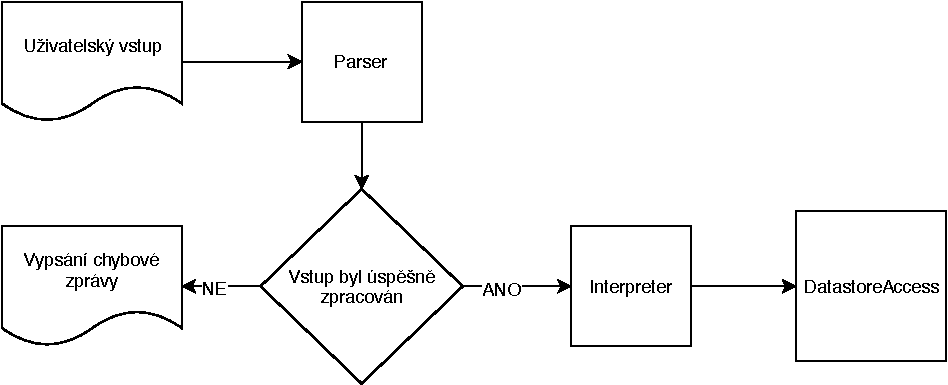
\includegraphics[width=.9\textwidth]{diagram}
\end{center}
\caption{Diagram proudu dat v programu}\label{proud:dat}
\end{figure}


\section{Uživatelské rozhraní}\label{ui}
Uživatelské rozhraní je poměrně přímočaré: program cyklicky načítá řádky uživatelského vstupu a zpracovává je. K interaktivnímu používání aplikace, je nutné implementovat funkci editace příkazové řádky. To zahrnuje především:
\begin{itemize}
    \item možnost úpravy aktuálního obsahu příkazové řádky před odesláním
    \item klávesové zkratky
    \item automatické doplňování příkazů
    \item ukládání historie příkazů
\end{itemize}
Ideální knihovna by měla mít nativní \Cpp{} rozhraní (ačkoliv lze v \Cpp{} relativně jednoduše použít i C knihovny) a být header-only, tedy, že k jejímu použití stačí přidat její hlavičkový soubor a všechny implementační detaily jsou obsaženy v něm.

Nejznámější knihovna využívaná k tomuto účelu je \textit{GNU Readline}\,\cite{readline}. \textit{Readline} umožňuje editaci příkazové řádky pomocí mnoha klávesových zkratek, převzatých z textových editorů \textit{EMACS} a \textit{Vi} a také velmi intuitivní inkrementální automatické doplňování (tj.\ postupné doplňování vícenásobným stisknutím klávesové zkratky). Nicméně, tato knihovna je již poměrně zastaralá, má pouze rozhraní v jazyce C, a tudíž vhodnou volbou pro moji aplikaci. Další nevýhodou je její implementace: \textit{Readline} obsahuje přibližně 20 tisíc řádek kódu především kvůli kompatibilitě s mnoha emulátory terminálů. V dnešní době většina terminálových aplikací podporuje základní VT100\footnote{terminál, jenž se stal předlohou pro novodobé terminálové aplikace} escape sekvence\footnote{kontrolní znaky, které slouží k ovládání terminálu; například mazání znaků nebo pohyb kurzorem} a tudíž není třeba zastaralé terminály podporovat.\cite{linenoise-readme}

Méně těžkotonážní variantou je knihovna \textit{linenoise}. Ta je oproti \textit{Readline} z hlediska velikosti zdrojového kódu velmi malá -- obsahuje zhruba tisíc řádků. Její odnož \textit{cpp-linenoise} je napsaná přímo v \Cpp{}, tudíž odpadají různé nevýhody použití knihovny s rozhraním v jazyce C, jako například absence podpory tříd\footnote{jazyk C není objektově orientovaný} a nutnost použití globálních proměnných.\footnote{například k definování funkce pro automatické doplňování} Zároveň je header-only. Z hlediska funkčních požadavků \textit{cpp-linenoise} bohužel zaostává: nepodporuje mnoho klávesových zkratek (například kombinace klávesy Ctrl a směrových šipek) a automatické doplňování je pouze velmi jednoduché (neinkrementální). Všechny tyto nedostatky řeší knihovna \textit{replxx}. Ta oproti \textit{linenoise} není header-only, nicméně velmi dobře napodobuje \textit{Readline} z hlediska podpory klávesových zkratek a automatického dokončování. Pro svůj program jsem tedy zvolil knihovnu \textit{replxx}.

\section{Zpracování vstupu pomocí \textit{Boost Spirit X3}}\label{spirit:intro}
Ke zpracování gramatik příkazů je potřeba parser.\footnote{syntaktický analyzátor; v mém programu část, která převádí textový vstup na strojově čitelný výstup} Implementaci parseru lze provést manuálně, to ovšem může být u složitých gramatik velmi nepraktické, a proto je vhodné použít nějakou knihovnu, která dokáže parser vygenerovat. Na základě konzultace s kolegou jsem použil knihovnu \textit{Boost Spirit X3}.

\subsection{\textit{Boost Spirit X3}}\todo{Možná nadpisy bez textit? YANG nadpis to třeba nemá}
\textit{Boost Spirit X3} je knihovna určená k vytváření parserů v jazyce \Cpp{}. Je součástí sady knihoven \textit{Boost}. Jednou z hlavních výhod \textit{Spiritu} je, že lze gramatiky zadávat přímo do zdrojového kódu výhradně pomocí prostředků jazyka -- operátorů\footnote{například plus, minus apod.} a \Cpp{} šablon. \Cpp{} umožňuje operátory předefinovat a tím změnit jejich funkcionalitu takřka libovolně. Důsledkem této vlastnosti je, že není potřeba spouštět žádný preprocesor\footnote{program, který transformuje zdrojový kód před jeho vlastním zpracováním}, který by převedl speciální syntaxi parseru do validního \Cpp{} kódu. V následujících kapitolách vysvětlím, jakým způsobem lze \textit{Spirit} používat.

\subsection{Základní pravidla}
\textit{Spirit} generuje parsery pomocí pravidel. Základními stavebními bloky jsou pravidla pro terminály. Příkladem může být pravidlo \verb¨int_¨, které parsuje jedno celé číslo, nebo \verb¨char_¨, které parsuje právě jeden znak. Kromě těchto pravidel, \textit{Spirit} definuje i složitější elementární pravidla jako třeba \texttt{alpha}, které slouží k parsování znaků abecedy nebo \texttt{digit}, které parsuje číslici. K parsování právě jednoho konkrétního znaku lze použít zápis znaku v \Cpp{} (například \verb¨'a'¨).

\subsection{Operátory}
Ke skládání pravidel ve \textit{Spiritu} slouží \Cpp{} operátory. Operátory lze různě kombinovat a zároveň funguje změna precedence operátorů pomocí závorek. Nyní popíšu funkci těch operátorů, které se v práci vyskytují.
\begin{description}
    \item[\uv{\texttt{>>}}]{Sekvence. \verb¨char_ >> char_¨ parsuje dva znaky za sebou. V EBNF se zapisuje pomocí čárky (\texttt{,}).}
    \item[\uv{\texttt{>}}]{\verb¨char_ > char_¨ parsuje dva znaky za sebou. Rozdíl oproti sekvenci spočívá v tom, že pokud se pravidlo za většítkem nezparsuje úspěšně, parsování automaticky končí neúspěchem. V EBNF neexistuje obdobný zápis.}
    \item[\uv{\texttt{*}}]{\verb¨*char_¨ parsuje jakýkoliv znak nula až nekonečně krát. V EBNF se pravidlo obaluje složenými závorkami.}
    \item[\uv{\texttt{+}}]{\verb¨+char_¨ parsuje jakýkoliv znak jednou až nekonečně krát. V EBNF neexistuje obdobný zápis.}
    \item[\uv{\texttt{prefixové -}}]{\verb¨-char_¨ parsuje jakýkoliv znak jednou nebo nula krát. V EBNF neexistuje obdobný zápis.}
    \item[\uv{\texttt{infixové -}}]{\verb¨char_-'a'¨ parsuje jakýkoliv znak kromě znaku \uv{a}. V EBNF se zapisuje stejně.}
    \item[\uv{\texttt{|}}]{Alternativa. \verb¨char_ | int_¨ parsuje jakýkoliv znak nebo číslo. V EBNF se zapisuje stejně.}
\end{description}

\subsection{Definice pravidel ve \textit{Spiritu}}
Definovat pravidla lze dvěma způsoby. Jeden z nich je pomocí tzv.\ \texttt{auto} pravidel. \texttt{auto} pravidla využívají \textit{type inference}, což je funkce \Cpp{}, která automaticky zjistí, o jaký typ proměnné se jedná a uživatel ho nemusí zadávat manuálně. Například deklarace \verb¨auto a = 0;¨ automaticky vyhodnotí, že datový typ proměnně \texttt{a} by měl být \texttt{int}. Vzhledem k tomu, že datový typ pravidel je takřka nemožné určit manuálně (název datového typu složitějších pravidel může mít kvůli šablonám i tisíce znaků), je tedy klíčové slovo \texttt{auto} téměř nezbytné. \texttt{auto} pravidla lze vidět na ukázkách~\ref{spirit:grammar}~a~\ref{spirit:nonterminals}. Pro jednoduché parsery často \texttt{auto} pravidla stačí. Pro složitější parsery je třeba použít pokročilou formu definice pravidel, o které se zmiňuji v kapitole~\ref{advanced:rules}.

\subsection{Srovnání zápisu v EBNF a ve \textit{Spiritu}}
K zápisu gramatik používá \textit{Spirit} syntaxi, která se podobá syntaxi EBNF\@. Rozdíl spočívá především ve využití operátorů, které nemají v EBNF obdobný zápis. Důsledkem je, že je gramatika zapsaná pomocí \textit{Spiritu} kratší. V ukázce~\ref{ebnf:quotedValues} je vidět EBNF gramatika, která odpovídá dvěma řetězcům, které jsou obalené uvozovkami.

\begin{itemize}
    \item Pravidlo \texttt{not-a-quote} je definováno jako výčet všech znaků kromě uvozovky.\footnote{vypisovat všechny znaky je velmi náročné, proto je pravidlo popsané pouze komentářem}
    \item Pravidlo \texttt{quotedValue} (\uv{uvozená hodnota}) je definováno jako zřetězení znaku uvozovky, alespoň jednoho znaku podle pravidla \texttt{not-a-quote}, poté libovolným množstvím znaků podle pravidla \texttt{not-a-quote} a nakonec jedním znakem uvozovka.
    \item Pravidlo \texttt{twoQuotedValues} řetězí dvě pravidla \texttt{quotedValue}.
\end{itemize}

\begin{listing}[H]
\begin{verbatim}
not-a-quote = ... (* všechny znaky kromě uvozovky oddělené svislou čarou *)
quotedValue = '"' , not-a-quote , {not-a-quote} , '"'
twoQuotedValues = quotedValue , quotedValue
\end{verbatim}
\caption{Příklad EBNF}\label{ebnf:quotedValues}
\end{listing}

Na ukázce~\ref{spirit:grammar} je stejná gramatika z ukázky~\ref{ebnf:quotedValues} zapsaná pomocí \textit{Spiritu}. Samotné pravidlo \verb¨'"'¨ říká, že pravidlo nejprve parsuje jednu uvozovku. Operátor \verb¨>>¨ značí sekvenci pravidel za sebou. \verb¨char:-'"'¨ znamená, že chceme parsenout jakýkoliv znak kromě uvozovky, a celé toto pravidlo je ještě obaleno operátorem \verb¨+¨, který celé vnitřní pravidlo zopakuje jednou až nekonečně krát (EBNF podporuje pouze nula až nekonečně krát). Na konci zbývá už jen pravidlo, které opět parsuje jednu uvozovku. Ve \textit{Spiritu} je každé takové pravidlo zároveň novým neterminálem a lze jej používat v jiných pravidlech stejně jako v EBNF\@. Pravidlo \texttt{twoQuotedValues} právě dvěma uvozeným řetězcům, definovaným v pravidlu \texttt{quotedValue}.

\begin{listing}[H]
\begin{minted}{c++}
auto const quotedValue = '"' >> +(char_-'"') >> '"';
auto const twoQuotedValues = quotedValue >> quotedValue;
\end{minted}
\caption{Příklad gramatiky napsané ve \textit{Spiritu}}\label{spirit:grammar}
\end{listing}


\subsection{Ukládání dat}
Abychom mohli pracovat s daty, které parser získá, je třeba je uložit do proměnných. K tomu ve \textit{Spiritu} slouží tzv.\ atributy pravidel. Atribut si lze představit jako datový typ návratových hodnot funkcí. Každé pravidlo má buď atribut \texttt{unused} (nevrací\footnote{\uv{vracením} je myšleno jaký atribut pravidlo vystavuje} nic), anebo některý z datových typů jazyka \Cpp{}. Příkladem může být jednoduché pravidlo \verb¨int_¨, které parsuje celé číslo a jeho atribut je datový typ \texttt{int}.

Pravidla ovšem nemusí vracet pouze primitivní datové typy, ale také celé datové struktury. U méně složitých pravidel dokáže \textit{Spirit} atribut odhadnout a není třeba ho explicitně definovat. Například pravidlo \verb¨+(char_-'"')¨ v ukázce~\ref{spirit:grammar} odpovídá řetězci (jednomu až mnoha znakům za sebou), a pro řetězce \textit{Spirit} určí datový typ \texttt{std::string}. Pravidlo \texttt{twoQuotedValues} odpovídá parsování dvou řetězců za sebou. V tomto případě již \textit{Spirit} návratový typ odhadnout nedokáže, a musíme ho zadat manuálně. V našem případě chceme uložit oba dva řetězce do dvou různých proměnných a ty sdružíme do \Cpp{} struktury, kterou můžeme vidět na ukázce~\ref{spirit:struct}. Tato struktura je s pravidlem kompatibilní, tzn.\ lze do ní uložit návratovou hodnotu tohoto pravidla.

\begin{listing}
\begin{minted}{c++}
struct TwoStrings {
    std::string firstString;
    std::string secondString;
}
\end{minted}
\caption{Kompatibilní struktura}\label{spirit:struct}
\end{listing}

\subsection{Pokročilá definice pravidel}\label{advanced:rules}
Pokud chceme kromě gramatiky pravidel nastavit i nějaké další parametry, \texttt{auto} pravidla už nestačí. V ukázce~\ref{spirit:advancedrule} je ukázán příklad kompletní definice pravidla. Nejprve definujeme proměnnou typu \texttt{x3::rule}, kterou se budeme na pravidlo odkazovat. První parametr šablony (\texttt{MyClass}) používá \textit{Spirit} interně k rozlišení pravidel a také slouží k definování různých vedlejších efektů, o kterých píšu v kapitole~\ref{sideeffects}. Druhý parametr šablony slouží k deklaraci atributu pravidla \texttt{TwoStrings}. Dále je třeba definovat gramatiku pravidla. To se dělá pomocí \textit{auto} pravidel, jejichž název končí na \verb¨_def¨. Nakonec je třeba registrovat pomocí makra \verb¨BOOST_SPIRIT_DEFINE¨.

\begin{listing}
\begin{minted}{c++}
x3::rule<MyClass, TwoStrings> const twoQuotedValues;

auto const quotedValue = '"' >> +(char_-'"') >> '"';
auto const twoQuotedValues_def = quotedValue >> quotedValue;

BOOST_SPIRIT_DEFINE(twoStrings)
\end{minted}
\caption{Pokročilá definice pravidla}\label{spirit:advancedrule}
\end{listing}

\subsection{Vedlejší efekty pravidel}\label{sideeffects}
Ačkoliv lze pomocí \textit{Spiritu} zapsat poměrně složité parsery, ne vždy může být jednoduché vytvořit gramatiku, která by ho generovala. Kvůli tomu \textit{Spirit} umožňuje na určitá místa vkládat kromě deklarativního\footnote{deklarativní kód je kód, kde programátor definuje, co má program udělat, ale ne jakým způsobem; to jsou například gramatiky ve \textit{Spiritu}} kódu i kód imperativní.\footnote{imperativní kód je kód, kde programátor určuje přesný postup algoritmu} Jedním ze způsobů, jak přidat imperativní kód je pomocí \uv{sémantických akcí}. Pomocí operátoru hranaté závorky (\verb¨[]¨) je možné k pravidlu přiřadit volatelný objekt (funkci, lambda funkci nebo funktor) a po úspěšném zparsování pravidla se objekt zavolá. V ukázce~\ref{spirit:semantic} lze vidět příklad použití. Pokud pravidlo úspěšně zparsuje číslo, program vypíše \uv{Hello, world!}.

\begin{listing}
\begin{minted}{c++}
auto const greeting = [] {
    std::cout << "Hello, world!" << std::endl;
};
auto const rule = int_[greeting];
\end{minted}
\caption{Sémantické akce}\label{spirit:semantic}
\end{listing}

Nevýhodou sémantických akcí je, že jejich používání velmi znepřehledňuje kód gramatik. Z tohoto důvodu existuje druhý způsob, jak přiřadit pravidlům imperativní kód a to pomocí \verb¨on_success¨ procedur. Zde hraje roli první parametr šablony \texttt{x3::rule}. Pokud do třídy, kterou v parametru uvedeme, nadefinujeme metodu \verb¨on_success¨, tato metoda se zavolá pří úspěšném zparsování pravidla podobným způsobem jako fungují sémantické akce. Výhodou je, že tímto způsobem oddělíme gramatiky od imperativního kódu a gramatiky se stanou čitelnějšími.

Kromě metody \verb¨on_success¨ lze ještě k pravidlům definovat metodu \verb¨on_error¨. Tato metoda se zavolá v případě, že gramatika daného pravidla nezparsovala pravidlo, které následovalo za operátorem většítko (\texttt{>}). V této metodě lze chybu odchytit, vypsat chybové hlášení a popřípadě i předat parseru další instrukce (například předat chybu u úroveň výš).

V ukázce~\ref{spirit:handler} můžeme vidět příklad jak zapsat třídu s \verb¨on_success¨ metodou. V této metodě máme k dispozici čtyři parametry, které poskytují informace o stavu parseru a také možnosti jak chování parseru ovlivnit:
\begin{description}
    \item[begin]{iterátor ukazující do místa ve vstupním řetězci, kde začalo parsování daného pravidla}
    \item[end]{iterátor ukazující do místa ve vstupním řetězci, kde skončilo parsování daného pravidla}
    \item[ast]{reference na atribut, který pravidlo vrací}
    \item[context]{parametr, pomocí kterého lze ovládat chování parseru}
\end{description}

\begin{listing}
\begin{minted}{c++}
struct greeting {
    template <typename T, typename Iterator, typename Context>
    inline void on_success(Iterator const& begin,
                           Iterator const& end,
                           T& ast,
                           Context const& context)
    {
        std::cout << "Hello, world!" << std::endl;
    }
}

x3::rule<greeting, int> const rule;

auto const rule_def = int_;
BOOST_SPIRIT_DEFINE(rule)
\end{minted}
\caption{Metoda \texttt{on\_success}}\label{spirit:handler}
\end{listing}

\section{Implementace syntaxe}\label{syntax:impl}
V následujících kapitolách se zabývám způsoby implementace syntaxe, která je popsána v kapitole~\ref{syntaxe}.

\subsection{Třída \texttt{Parser}}
Rozhraní parseru je implementováno pomocí třídy \texttt{Parser}. Úkolem této třídy je volání metod knihovny \textit{Spirit} a využívání vytvořených gramatik k parsování vstupu a automatickému doplňování. Je v ní také uložen aktuální kontext programu.

Nejdůležitější metodou je \texttt{parseCommand}, jejíž vstupním parametrem je řetězec, který chceme parsovat a vrací datovou strukturu odpovídající uživatelskému vstupu. Dále se zde nachází metoda \texttt{completeCommand}, která funguje takřka stejně jako \texttt{parseCommand}, ale místo datové struktury vrací seznam možných dokončení příkazu. Metoda \texttt{changeNode} slouží ke změně kontextu (pomocí příkazu \texttt{cd}) a metoda \texttt{availableNodes} vrací všechny poduzly v aktuálním kontextovém uzlu.

\subsection{Metoda \texttt{parseCommand}}
Tato metoda obstarává volání vygenerovaného \textit{Spirit} parseru na uživatelský vstup. Jejím úkolem je také vytvoření instance třídy \texttt{ParserContext}, o které píšu v kapitole~\ref{path:checking}. Volání vygenerovaného \textit{Spirit} parseru probíhá pomocí funkce \texttt{x3::phrase\_parse}. Tato funkce přijímá několik parametrů:

\begin{itemize}
    \item referenci na iterátor, který odpovídá začáku vstupního řetězce
    \item iterátor, který odpovídá konci vstupního řetězce
    \item gramatiku, podle které bude parsování probíhat
    \item \uv{skip parser}, který určuje, které znaky parser přeskakuje
    \item referenci na výstupní strukturu
\end{itemize}
První dvojice iterátorů definuje začátek a konec vstupu.\footnote{vstup je typu \texttt{std::string}; lze ho definovat pomocí iterátoru na začátek a konec} První argument je datového typu reference z toho důvodu, že \textit{Spirit} tento iterátor iterně používá k pohybu nad vstupním řetězcem. To znamená, že po dokončení zpracování lze zjistit, na jakém místě parsování skončilo.

\uv{Skip parser} je speciální parserm, který určuje, které znaky parser přeskočí\footnote{ve \textit{Spiritu} existuje i funkce \texttt{x3::parse}, která tuto funkci nemá} přeskakuje. Výhoda přeskakování je, že se gramatiky programu nemusí starat o mezery a parser jich přeskočí libovolný počet.

Posledním argumentem\footnote{funkce je variadická, což znamená, že lze použít i více výstupních parametrů} je reference na výstupní strukturu. Do této struktury se ukládá strojově čitelný výstup, jenž je výsledkem celého parsování. Ke každému netriviálnímu pravidlu\footnote{triviálními pravidly jsou myšleny například pravidla, která parsují přímo jednotlivé znaky (v jejich gramatikách se neobjevují neterminály)} je vytvořena odpovídající struktura. Například pro datovou cestu je vytvořena struktura \texttt{dataPath\_}, pro schematickou cestu struktura \texttt{schemaPath\_} atd. Struktury na nejvyšší úrovni odpovídají jednotlivým příkazům. To znamená, že pro každý příkaz je vytvořena právě jedna struktura, která ho jednoznačně definuje. Ukázka~\ref{struct:cd} ukazuje definici struktury pro příkaz \texttt{cd\_}. Výstupní parametr parseru má tedy datový typ, který dokáže obsáhnout kteroukoli z těchto struktur. Standardní knihovna \Cpp{} nabízí k tomuto účelu třídu \texttt{std::variant}, nicméně z důvodů popsaných v kapitole~\ref{completing:commands} jsem zvolil třídu \texttt{boost::variant}.

\begin{listing}
\begin{minted}{c++}
struct cd_ : x3::position_tagged {
    dataPath_ m_path;
};
\end{minted}
\caption{Struktura \texttt{cd\_}}\label{struct:cd}
\end{listing}

Pokud parsování neproběhlo úspěšně, metoda \texttt{parseCommand} vyvolává výjimku. Součástí parsování jsou i chybové výpisy, které se vypisují na proud\footnote{například standardní výstup nebo standardní chybový výstup}, který je metodě předáván, jako druhý parametr.

\subsection{Gramatiky příkazů}
Vytvořit gramatiky samotných příkazů podle jejich syntaxe je poměrně jednoduché. Nejsložitější gramatiku má příkaz \texttt{ls}, kterou lze vidět v ukázce~\ref{grammar:ls}. Nejprve gramatika parsuje řetězec \verb¨"ls"¨ (uložený v proměnné \verb¨ls::name¨). Nyní je potřeba zparsovat volitelný přepínač \verb¨ls_options¨. Samotné pravidlo pro tento přepínač je uvedeno v ukázce~\ref{grammar:ls:options}. Toto pravidlo je implementováno pomocí \uv{symbol table}, což je způsob, jak definovat, které řetězce se mají zparsovat a jaké budou jejich atributy. V ukázce vidíme, že jediný přepínačem je přepínač \verb¨--recursive¨ a při jeho úspěšném zpracování vrací pravidlo konstantu \texttt{LsOption::Recursive} (definovanou v jiné části programu).

\begin{listing}
\begin{minted}{c++}
auto const ls_def =
    ls_::name >> *(space_separator >> ls_options)
    >> -(space_separator >> (dataPathListEnd |
                             dataPath |
                             schemaPath));
\end{minted}
\caption{Gramatika příkazu \texttt{ls}}\label{grammar:ls}
\end{listing}


\begin{listing}
\begin{minted}{c++}
struct ls_options_table : x3::symbols<LsOption> {
    ls_options_table()
    {
    add
        ("--recursive", LsOption::Recursive);
    }
} const ls_options;
\end{minted}
\caption{Pravidlo \texttt{ls\_options}}\label{grammar:ls:options}
\end{listing}

Dále je nutné zajistit, aby program vyžadoval mezery mezi jednotlivými fragmenty příkazu. To zajišťuje pravidlo \verb¨space_separator¨, které je možné vidět na ukázce~\ref{grammar:space:separator}. Důvodem, proč je pravidlo poněkud složitější, je, že způsob, jakým v programu parsuji příkazy automaticky přeskakuje mezery (využívám výše zmíněnou funkci \texttt{phrase\_parse}). Tomu lze manuálně zabránit direktivou \verb¨x3::no_skip¨. Direktivy obalují pravidla a mění jejich vlastnosti, v tomto případě vypnutí přeskakování mezer. Druhou použitou direktivou je \verb¨x3::omit¨, která způsobí, že se zahodí atribut pravidla. Pravidlo \texttt{space} je součástí \texttt{Spiritu} a odpovídá jednomu \uv{bílému}\footnote{mezeře, tabulátoru nebo novému řádku} znaku.

\begin{listing}
\begin{minted}{c++}
auto const space_separator =
    x3::omit[x3::no_skip[space]];
\end{minted}
\caption{Pravidlo \texttt{space\_separator}}\label{grammar:space:separator}
\end{listing}

Nakonec je třeba zapsat gramatiku pro argument cesty. Vzhledem k tomu, že \texttt{ls} přijímá jakoukoli cestu, v gramatice jsou jako alternativy vypsány všechny druhy cest. O implementaci pravidla pro cesty mluvím v následující kapitole.

\subsection{Gramatiky cest}
Implementace syntaxe pro cesty je nejsložitější gramatikou z celého programu. Důvodem je to, že názvy uzlů v cestě se mění na základě modelů \textit{YANG} a program je musí kontrolovat dynamicky. Vzhledem k tomu, že pravidla jsou pevně daná a neexistuje mnoho prostředků pro vytváření dynamických pravidel, rozhodl jsem se provést kontrolu názvů uzlů pomocí imperativního kódu, který zakomponuji do \verb¨on_success¨ metod jednotlivých pravidel.

Nejprve ale k samotným gramatikám. Gramatika pro schematickou cestu cestu vypadá takto:
\begin{minted}{c++}
auto const schemaPath_def =
    initializePath >> absoluteStart >> createPathSuggestions >>
    x3::attr(decltype(schemaPath_::m_nodes)()) >>
    x3::attr(TrailingSlash::NonPresent) >> x3::eoi
    |
    initializePath >> -(absoluteStart >> createPathSuggestions) >>
    schemaNode % '/' >> (trailingSlash >> createPathSuggestions >>
    (completing | x3::eoi) | (&space_separator | x3::eoi));

\end{minted}
Celé pravidlo pro schematickou cestu je rozdělené do dvou větví (pomocí operátoru \texttt{|}). První větev odpovídá samotnému lomítku -- tedy, když chce uživatel zadat jako cestu kořen stromu. Druhá větev odpovídá cestě, v které je alespoň jeden uzel.

Hlavní částí první větve je pravidlo \texttt{absoluteStart}. Je velmi jednoduché -- parsuje lomítko a jeho atribut je příznak, který říká, že uživatel zadal absolutní cestu.\footnote{z hlediska \uv{absolutnosti} je cesta, která obsahuje pouze lomítko absolutní} Druhé pravidlo, které je zde důležité je \texttt{x3::eoi}. To způsobuje, že větev bude platná pouze pokud uživatel lomítko a žádný další vstup. Protože samotná větev parsuje jen lomítko, je třeba ještě manuálně dodat takové atributy, aby byla větev kompatibilní se strukturou \texttt{schemaPath\_}.

Druhá větev parsuje názvy uzlů pomocí pravidla \verb¨schemaNode \% '/'¨. Operátor procento (\texttt{\%}) parsuje seznamy oddělené znakem. Například pravidlo \verb¨'a' % ','¨ parsuje znaky \texttt{a} oddělené čárkami. Na ukázce se tedy parsuje několik řetězců, které podléhají pravidlu \texttt{schemaNode} a které jsou odděleny lomítkem. To odpovídá stanovené syntaxi cest. Zbylá pravidla jsou pouze \uv{pseudopravidla}. Jejich gramatiky nic neparsují\footnote{obsahují pouze \texttt{x3::eps}, neboli epsilon, tedy prázdný řetězec} a slouží pouze k zavolání imperativního kódu. Pomocí těchto pravidel je také implementováno automatické doplňování, o kterém mluvím v kapitole~\ref{completion}.

Pravidlo \texttt{schemaNode} parsuje jednotlivé názvy uzlů. Jeho gramatika vypadá takto:
\begin{minted}{c++}
auto const schemaNode_def =
createPathSuggestions >> -(module) >> (container |
                                       list |
                                       nodeup |
                                       leaf);
\end{minted}
Zde lze již vidět některé konstrukty \textit{YANG}. Za pravidly \texttt{container}, \texttt{list} a \texttt{leaf} se skrývají gramatiky, které určují platný název uzly v modelu \texttt{YANG}. Liší se především v jejich \verb¨on_success¨ metodách. V těchto metodách probíhá zmiňovaná dynamická kontrola názvů (a druhů) uzlů. V následujících podkapitolách popisuji, jakým způsobem je tato kontrola implementována.

\subsubsection{Rozhraní \texttt{Schema}}
Ke kontrole cest slouží abstraktní rozhraní \texttt{Schema}. Toto rozhraní obsahuje různé metody pro kontrolu cest jako například \texttt{isLeaf}, která zjišťuje, jestli je uzel s danou cestou uzel typu \texttt{leaf}. Konkrétně je toto rozhraní implementováno jako třída \texttt{StaticSchema}, která je určená k testování, a jako třída \texttt{YangSchema}, která využívá knihovnu \textit{libyang}~\cite{libyang}. \textit{Libyang} je knihovna vytvořená spoečností CESNET, která umožňuje manipulovat s modely \textit{YANG}.

\subsubsection{Kontrola cest}\label{path:checking}
Kontrola cest probíhá v \verb¨on_success¨ metodách pravidel pro jednotlivé typy uzlů. Pomocí direktivy \texttt{x3::with} umožňuje \textit{Spirit} vložit do gramatiky jakýkoliv objekt, který lze poté v těchto metodách získat pomocí funkce \texttt{x3::get}. Pro kontrolu cest by stačilo do startovacího pravidla\footnote{pravidlo, kde jsou sdruženy pravidlo pro všechny příkazy} vložit objekt typu \texttt{Schema}, nicméně je třeba, aby parser propagoval i nějaké další informace (kromě samotných příkazů) zpět. Proto jsem vytvořil třídu \texttt{ParserContext}, která obsahuje mimo jiné několik proměnných, které jsou potřebné pro validaci cest. Jedna z nich je rozhraní \texttt{Schema} a další je aktuální uzel, v kterém se parser nachází.

Implementace metod je poté poměrně přímočará -- v závislosti na typu uzlu se zavolá příslušná metoda (např.\ \texttt{isLeaf}) rozhraní Schema. Pokud rozhraní vrátí pozitivní odpověď, je název uzlu přijat a parsování pokračuje. Pokud bude odpověď negativní je třeba parser zastavit.

Ukázka~\ref{on:success} ukazuje, jak vypadá \verb¨on_success¨ metoda třídy \texttt{leaf\_class}. Nejprve metoda získá pomocí \texttt{x3::get} vloženou instanci \texttt{ParserContext}, poté zavolá metodu \texttt{isLeaf} s aktuálním uzlem a na základě výsledku může parseru říct, že pravidlo ve skutečnosti neproběhlo úspěšně (pomocí \verb¨_pass(context) = false;¨).

\begin{listing}[H]
\begin{minted}{c++}
struct leaf_class {
template <typename T, typename Iterator, typename Context>
void on_success(Iterator const&,
                Iterator const&,
                T& ast,
                Context const& context)
{
    auto& parserContext = x3::get<parser_context_tag>(context);
    const auto& schema = parserContext.m_schema;

    if (!schema.isLeaf(parserContext.m_curPath,
                       {parserContext.m_curModule, ast.m_name}))
        _pass(context) = false;
}
};
\end{minted}
\caption{\texttt{on\_success} metoda pro \texttt{leaf}}\label{on:success}
\end{listing}

\section{Automatické doplňování}\label{completion}
Jednou z klíčových součástí mého programu je automatické doplňování příkazů a jejich argumentů.\footnote{doplňování není plně automatické, protože uživatel musí pro doplnění zmáčknout klávesu} Tato funkce je stěžejním prvkem pro dosažení uživatelské přívětivosti programu. V následujících kapitolách popisuji, co vše lze v aplikaci doplňovat a také způsoby, které jsem použil k implementaci doplňování.

\subsection{Vyvolání doplňování}
O samotnou úpravu uživatelského vstupu a odchycení klávesy tabulátor, jakožto klávesové zkratky, se stará knihovna \textit{replxx}. Na ukázce~\ref{replxx:callback} je vidět, jakým způsobem se používá metoda \texttt{set\_completion\_callback} pro registraci vlastní funkce pro doplňování. Tato metoda přijímá volatelný objekt, s parametrem vstupu, který vrací \texttt{std::vector}\footnote{\Cpp{} kolekce proměnných stejného datového typu} řetězců, kterými lze vstup doplnit.

\begin{listing}[H]
\begin{minted}{c++}
lineEditor.set_completion_callback(
[&parser](const std::string& input, int&) {
    std::stringstream stream;
    auto completionsSet = parser.completeCommand(input, stream);

    std::vector<std::string> res;
    std::transform(completionsSet.begin(),
                   completionsSet.end(),
                   std::back_inserter(res),
                   [input](auto it) { return it; });
    return res;
});
\end{minted}
\caption{Registrace doplňující funkce}\label{replxx:callback}
\end{listing}

\subsection{Metoda \texttt{completeCommand}}
Generování doplňovacích řetězců (návrhů) probíhá v metodě \texttt{completeCommand}. Vstupní řetězec se parsuje stejným způsobem jako při použití metody \texttt{parseCommand}, ale při volání funkce \texttt{phrase\_parse} se výstupní strkutura zahazuje. Místo toho slouží jako výstupní hodnota proměnná \texttt{m\_completions} v třídě \texttt{ParserContext}. Do této proměnné se pomocí speciálních \uv{pseudopravidel} ukládají návrhy na doplnění příkazů. V závislosti na tom, kdy parsování končí (nemusí končit úspěšně, jelikož nemusím vždy doplňovat kompletní příkaz), se použijí poslední vygenerované návrhy.

Vzhledem k tomu, že parser generuje návrhy jen v určitých momentech (například mezi jednotlivými názvy uzlů) a parser nezpracuje vždy celý vstup, je třeba implementovat filtrování návrhů. Toto se děje pomocí pomocné funkce \texttt{filterByPrefix}.

\subsection{Pseudopravidla}
\uv{Pseudopravidla} jsou v mých gramatikách pravidla, která neslouží k parsování vstupu, ale pouze jako řídící struktury parseru. Jejich gramatikou je vždy pouze \texttt{x3::eps}. Z tohoto důvodu se vždy provedou jejich \texttt{on\_success} handlery a tímto způsobem je možné vkládat do gramatiky imperativní kód. Pseudopravidla používám k vytváření návrhů na doplňování a také na inicilizaci některých proměnných obsažených ve třídě \texttt{ParserContext}.


\subsection{Doplňování názvů příkazů}\label{completing:commands}
Jeden z podporovaných doplňování je dokončení názvu příkazů, jehož implementace se nachází v pravidle \texttt{createCommandSuggetions}. Jeho \texttt{on\_success} je poměrně přímočarý: pomocí funkce \texttt{for\_each} knihovny \textit{Boost MPL}\cite{boost:mpl} iteruji výsledný datový typ\footnote{výsledným datovým typem je myšlen \texttt{boost::variant} všech struktur příkazů (\texttt{cd\_}, \texttt{ls\_}, \ldots); iterací je myšlena iterace přes všechny tyto struktury} celého parseru. Každá struktura asociovaná s příkazem má v sobě také uložený řetězec s názvem příkazu (například \verb¨"cd"¨). V ukázce~\ref{createCommandSuggetions} je vidět, že ačkoliv kód neprovádí mnoho, využití knihovny \textit{MPL} celý kód poměrně znepřehledňuje to takový kód dělá. Nutnost použití knihovny \textit{MPL} vyplývá z toho, že \textit{Spirit} zatím nepodporuje standardní typ \texttt{std::variant}~\cite{boost-variant}, který umožňuje iterovat obsažené datové typy bez použití knihovny třetí strany.

\begin{listing}
\begin{minted}{c++}
boost::mpl::for_each<CommandTypes, boost::type<boost::mpl::_>>(
    [&parserContext](auto cmd) {
        parserContext.m_suggestions.emplace(commandNamesVisitor()(cmd));
});
\end{minted}
\caption{Iterace datových typů \texttt{boost::variant}}\label{createCommandSuggetions}
\end{listing}


\subsection{Doplňování cest}
Kromě názvů příkazů je také možné doplňovat cesty k uzlům. Tato funkce je implementována v pseudopravidlu \texttt{createPathSuggestions}. Z hlediska gramatiky, generování cest probíhá vždy mezi jednotlivými uzly. K získání uzlů pro doplnění slouží metoda \texttt{childNodes}, obsažena v rozhraní \texttt{Schema}, které je součástí pomocné třídy \texttt{ParserContext}.

Poté, co parser vygeneruje návrhy cest, mohou nastat tři situace. U každé situace je ukázka, která znázorňuje, jaký je stav parseru po dokončení parsování.
\begin{enumerate}
    \item Po parsování na vstupu nezbyly žádné znaky.

        V tomto případě není třeba návrhy filtrovat a návrhy jsou zobrazeny v původní podobě: pokud by existovala validní cesta \texttt{first/second} a uživatel by chtěl doplnit příkaz \texttt{cd first/second/}, celý vstup by se zpracoval a výslednými návrhy by byly poduzly obsažené v uzlu \texttt{first/second}.
        \begin{verbatim}
        /> cd first/second/
                          ^ parser skončil zde
        \end{verbatim}
    \item Po parsování na vstupu zbyly znaky, které nebyl parser schopný parser zpracovat.

        Nezpracované znaky na konci vstupu mohou potencionálně znamenat začátek dalšího uzlu. Vzhledem k tomu, že lze jednoduše zjistit, kde přesně parser skončil, je jednoduché použít nezpracované znaky pro vyfiltrování návrhů. Například, pokud by existovaly validní cesty \texttt{first/second}, \texttt{first/service} a \texttt{first/something} a uživatel bude chtít doplnit příkaz \texttt{cd first/se}. V tomto případě by \uv{se} zůstalo nezpracované a program zobrazí návrhy \uv{second} a \uv{service}.
        \begin{verbatim}
        /> cd first/se
                   ^ parser skončil zde
        \end{verbatim}
    \item Po parsování na vstupu nezbyly žádné znaky, ale aktuální vstup lze pořád doplnit.

        Například, pokud by existovaly validní cesty \texttt{first/min} a \texttt{first/minister} a uživatel zadá příkaz \texttt{cd first/min}. V tento moment může uživatel buď příkaz potvrdit (jelikož \texttt{first/min} je validní cesta), anebo vygenerovat návrhy a případně zvolit cestu \texttt{first/minister}. Tento případ se liší od situace 2 tím, že parser zpracoval veškerý vstup. To znamená, že nemohu použít řetězec \texttt{min} pro filtrování návrhů (protože parser zpracoval veškerý vstup). Kdyby uzel \texttt{first/min} neexistoval, parser by se zastavil už na lomítku. Je tedy nutné zjistit, kde přesně byly návrhy vygenerovány.
        \begin{verbatim}
        /> cd first/min
                      ^ parser skončil zde
        \end{verbatim}

        \textit{Spirit} do \texttt{on\_success} metod předává několik parametrů. Jeden z nich je parametr \texttt{begin}, který říká, kde se momentálně parser ve vstupním řetězci nachází. Tuto informaci předám pomocí třídy \texttt{ParserContext} zpět do metody \texttt{completeCommand}, kde ji využívám k filtrování výsledků.
\end{enumerate}

\subsection{Doplňování hodnot typu identityref a enumeration}
Při nastavování hodnot příkazem \texttt{set} uživatel nemusí přesně vědět jaké hodnoty jsou pro daný \texttt{leaf} povolené. U datových typů jako celé číslo nebo řetězec, kde může být hodnota libovolná nemá doplňování smysl, nicméně u datových typů, kde jsou povolené hodnoty součástí nějaké uzavřené množiny, to smysl má. Dva z takových typů jsou typ identityref a typ enumeration. Tyto hodnoty se generují pomocí pseudopravidel \texttt{createEnumSuggestions} a \texttt{createIdentitySuggestions}.

V ukázce~\ref{leaf:enum} je definice \texttt{leafu} s typem enumeration, který reprezentuje druh pizzy. Tento \texttt{leaf} může nabývat pouze hodnot definovaných pomocí definic \texttt{enum}.

Datový typ identityref je poněkud složitější. Identity se definují mimo uzly a lze volitelně definovat tzv.\ \uv{base identitu}. Na ukázce~\ref{leaf:identityref} existuje například base identita \texttt{interface\_base} a identita \texttt{ethernet}, jejíž base identita je právě \texttt{interface\_base}. \texttt{leaf} s názvem \texttt{network\_card}, který je datového typu identityref také definuje svoji base identitu. Platnými hodnotami pro tento \texttt{leaf} jsou všechny identity, jejichž base identita je \texttt{interface\_base}.

\begin{listing}[H]
        \begin{minted}{c++}
leaf pizza {
    type enumeration {
        enum hawaii;
        enum margherita;
        enum pollo;
    }
}
\end{minted}
\caption{Definice \texttt{leafu} typu enumeration}\label{leaf:enum}
\end{listing}

\begin{listing}[H]
\begin{minted}{c++}
identity password;
identity interface_base;
identity ethernet {
    base interface_base;
}
identity wifi {
    base interface_base;
}
leaf network_card {
    type identityref {
        base interface_base;
    }
}
\end{minted}
\caption{Definice \texttt{leafu} typu identityref}\label{leaf:identityref}
\end{listing}



\subsection{Doplňování klíčů instancí \texttt{listů}}
Uživatel nemusí vždy vědět, jaké klíče jsou potřeba k jednoznačné definici instance \texttt{listu}. Z tohoto důvodu parser v určitých momentech doplňuje hranaté závorky a názvy klíčů. Při doplňování klíčů mohou nastat dvě situace:

\begin{enumerate}
    \item Uživatel zadal kompletní název \texttt{listu} a neexistuje žádný jiný uzel, která by začínal stejným názvem.

        V tento moment aplikace doplňuje levou hranatou závorku (\verb¨[¨). Ukázka:
        \begin{verbatim}
        /> set example:list
        /> set example:list[
        \end{verbatim}

    \item Uživatel zadal kompletní název \texttt{listu}, ale existuje jiný uzel, jehož název začíná jako zmiňovaný list.

        Aplikace v tuto chvíli neví, jestli uživatel chce chce doplnit závorku a začít zadávat klíče, nebo chce, aby program doplnil název uzlu. Program tedy musí nabídnout obě varianty. Ukázka:
        \begin{verbatim}
        /> set example:list
        example:list example:listing
        /> set example:list
        \end{verbatim}

\end{enumerate}
Tyto situace lze rozlišit podle toho, jestli je doplnění jednoznačné (tj.\ že po filtrování zůstane jen jeden návrh). Vzhledem k tomu, že filtrování návrhů probíhá mimo parser, metoda \texttt{completeCommand} neví, co doplnit, pokud se ukáže, že návrh zůstal jen jeden. Kvůli tomu jsem vytvořil ve třídě \texttt{ParserContext} proměnnou \texttt{m\_completionSuffix}. Do této proměnné parser zapíše, co se má k návrhu připsat za předpokladu, že bude jen jeden.


\section{Interpretace příkazů}\label{interpreter}
Poté, co data opustí parser ve formě strojově čitelných struktur, je třeba příkazy vykonat (interpretovat). K tomu slouží třída \texttt{Interpreter}, jejíž design odpovídá návrhovému vzoru \textit{visitor}. Principem tohoto návrhového vzoru je oddělit data a funkcionalitu, která je nad těmito daty prováděna. V tomto případě jsou tato data struktury, které získávám pomocí knihovny \textit{Spirit}. Třída \texttt{boost::variant}, jenž je datovým typem výsledné struktury knihovny \textit{Spirit}, podporuje tento návrhový vzor nativně pomocí funkce \texttt{boost::apply\_visitor}.

V \Cpp{} se \textit{visitor} implementuje pomocí přetížení operátoru závorky (\texttt{()}). Použití třídy \texttt{Interpreter} je vidět v ukázce~\ref{interpreter:invocation}. Metoda \texttt{parseCommand} nejprve vytvoří výslednou strukturu. Funkce \texttt{boost::apply\_visitor} přijímá dva parametry: instanci třídy, která podléhá vzoru \textit{visitor} (zde je vždy vytvořena nová instance), a proměnnou typu \texttt{boost::variant}, s kterou bude \textit{visitor} použit. Tato funkce zavolá na \textit{visitor} operátor závorky s argumentem, který jsme předali jako druhý. Celý tento kód je obalen blokem \texttt{try}, který případě odchytí výjimku vyvolanou metodou \texttt{parseCommand}.

\begin{listing}
\begin{minted}{c++}
try {
    command_ cmd = parser.parseCommand(line, std::cout);
    boost::apply_visitor(Interpreter(parser, datastore), cmd);
} catch (InvalidCommandException& ex) {
    // handle error
}
\end{minted}
\caption{Volání interpreteru}\label{interpreter:invocation}
\end{listing}

\texttt{Interpreter} slouží pouze jako mezivrstva, která spojuje uživatelské rozhraní a úložiště konfigurace. Jeho implementace spočívá v tom, že pro každý příkaz je přetížený operátor závorky. Pro příkazy bez parametrů je kód velmi přímočarý, jak je vidět na ukázce~\ref{interpreter:commit:discard} -- spočívá v zavolání jediné metody rozhraní \texttt{DatastoreAccess}. Složitější příkazy již potřebují měnit své chování v závislosti na parametrech příkazů. Jeden z nich je příkaz \texttt{ls}, který podporuje přepínač \verb¨--recursive¨. Na toto musí interpreter příslušně reagovat.

\begin{listing}
\begin{minted}{c++}
void Interpreter::operator()(const commit_&) const {
    m_datastore.commitChanges();
}
void Interpreter::operator()(const discard_&) const {
    m_datastore.discardChanges();
}
\end{minted}
\caption{Interpretace příkazů \texttt{commit} a \texttt{discard}}\label{interpreter:commit:discard}
\end{listing}

Třída \texttt{Interpreter} dále obsahuje různé pomocné metody, které jsou potřeba k interpretaci příkazů. Jednou z nich je metoda \texttt{absolutePathFromCommand}, která převádí strojově čitelnou reprezentaci cest zpět na řetězce. Datové struktury mého programu reprezentující cesty obsahují sice více informací (např.\ typy uzlů), nicméně komunikace s datovými úložišti probíhá výhradně pomocí textových řetězců, tudíž je třeba struktury převést.


\section{Přístup k úložišti konfigurace}\label{datastore:access}
Třída \texttt{Interpreter} používá pro přístup k datovému úložišti rozhraní \texttt{DatastoreAccess}. Součástí tohoto rozhraní jsou metody určené k získávání a odesílání konfigurace na vzdálený server. Výhodou volby abstraktního rozhraní je, že třída \texttt{Interpreter} nezávisí na konkrétním implementace přenosu dat mezi datovým úložištěm a implementovaným programem. To znamená, že se implementovaný program může připojit k jakémukoliv typu datového úložiště (podmínkou ovšem je, že musí používat k validaci modely \textit{YANG}). Kromě protokolu \textit{NETCONF} používá \textit{YANG} k validaci konfigurace i program \textit{sysrepo}\,\cite{sysrepo}.

\subsection{SysrepoAccess}
Před implementací komunikace pomocí protokolu \textit{NETCONF} bylo třeba vyladit parser a uživatelské rozhraní. Z tohoto důvodu jsem nejprve implementoval třídu \texttt{SysrepoAccess}, která komunikuje pomocí klientské knihovny \textit{sysrepo}. Použití této knihovny je velmi jednoduché: odpadá jakákoliv nutnost znalosti \textit{NETCONFu}. \textit{Sysrepo} pomocí tohoto protokolu nekomunikuje. Rozhraní \textit{sysrepa} je poměrně přímočaré: pro nastavování hodnot libovolných uzlů slouží metoda \texttt{sysrepo::set\_item}. Naopak, pro získání konfigurace slouží metoda \texttt{sysrepo::get\_items}. Kvůli jednoduchosti tohoto rozhraní jsem při návrhu a testování nemusel řešit, jakým způsobem způsobem funguje protokol \textit{NETCONF}.

\subsection{NetconfAccess}
% TODO: I'm fucked. NOT IMPLEMENTED. I'll try to complete the implementation later...


\chapter{Vyhodnocení}
V první části této kapitoly se zabývám tím, jaké technologie jsem použil pro otestování aplikace. V druhé části porovnávám svoji aplikaci s existujícími řešeními, popisuji její výhody a kontroluji splnění cílů.
\section{Testování}
Testování aplikace na úrovni kódu probíhalo již od začátku vývoje díky systému \textit{continuous integration}. \textit{Continuous integration} umožňuje automatické spouštění testů po nahrání nové verze kódu na serveru a pokud server zjistí, že nějaký test neproběhl úspěšně, označí novou verzi jako chybnou a je třeba chybu opravit. Při vývoji jsem používal metodu \textit{TDD}.\footnote{test-driven development} Principem této metody je, že před implementací nové funkce se nejdřív vytvoří test, který popisuje očekávané chování nové funkce. S téměř\footnote{některé funkce lze jen velmi těřko testovat -- např.\ uživatelské rozhraní} každou novou funkcí byl tedy přidán i příslušný test.

K testování jsem nejprve používal knihovnu \textit{Catch}\,\cite{catch2}. Výhoda knihovny \textit{Catch} je, že společné části jednotlivých testů lze definovat pouze jednou. Rozdílné části se definují pomocí maker \texttt{SECTION}. Na ukázce~\ref{catch:example} je vidět část testu s makry \texttt{SECTION}. V tomto případě testuji pomyslnou funkci \texttt{isEven}, která zjišťuje, jestli je číslo sudé. V tomto testu se nachází dvě větve. To zajíšťuje, že se test vykoná dvakrát, jednou průběhem jednou větví a podruhé větví druhou. Vytvoření proměnné \texttt{a} je společné pro obě větve.

V pozdější fázi vývoje jsem přešel na knihovnu \textit{doctest}\,\cite{doctest}, který téměř stejné rozhraní jako knihovna \textit{Catch2}. Výhodou knihovny \textit{doctest} je, že s jejím použitím se testy kompilují mnohem rychleji, než při použití knihovny \textit{Catch2}.

\begin{listing}
\begin{minted}{c++}
TEST_CASE("isEven")
{
    int a;
    SECTION("větev první")
    {
        a = 2;
    }

    SECTION("větev druhá")
    {
        a = 10;
    }
    REQUIRE(isEven(a));
}
\end{minted}
\caption{Ukázka testování pomocí knihovny \texttt{Catch2}}\label{catch:example}
\end{listing}

\subsection{Testování parseru}
Nejdůležitější součást -- parser -- je testována nejvíce. Testů je mnoho a jsou rozděleny do několika souborů. Příkladem je například soubor \texttt{cd.cpp}, který specificky testuje zpracovávání příkazu \texttt{cd} nebo soubor \texttt{leaf\_editing.cpp}, který testuje parsování příkazu \texttt{set}. Pro otestování parseru byla pro zjednodušení implementována třída \texttt{StaticSchema}, která napodobuje třídu \texttt{YangSchema}.

Testuje se jak pomocí \uv{pozitivních} testů, tak \uv{negativních} testů. V pozitivních testech je metodě \texttt{parseCommand} předán textový vstup s validním příkazem. Metoda nesmí při testu vyvolat výjimku a výstupní struktura parseru musí odpovídat očekávané struktuře definované v každém testu. V negativních testech je naopak metodě předán neplatný příkaz. V tomto případě musí metoda vyvolat výjimku.

Kromě samotného parsování se rovněž testuje schopnost parseru generovat návrhy na doplňování. Testování doplňování je velmi důležité, neboť doplňování je klíčovou vlastností implementovaného programu. Většina funkcí, o kterých jsem psal v kapitole~\ref{completion}, je tudíž řádně otestována.

\subsection{Unit testy třídy \texttt{YangSchema}}
Aby byla zajištěna správná funkčnost třídy \texttt{YangSchema}, je tato třída testována pomocí \textit{unit testů}. Unit testy jsou jednoduchou metodou jak otestovat jednu elementární část programu. Každá metoda v této třídě je testována na příkladovém modelu \textit{YANG}. Opět se zde vyskytují pozitivní i negativní testy.


\section{Porovnání s existujícími řešeními}
Nevýhodou programů, které implementují komunikaci pomocí protokolu \textit{NETCONF}, o kterých jsem psal v kapitole~\ref{existing} je, že pohlížejí na komunikaci tak, jak funguje komunikace přes \textit{NETCONF}. Důsledkem toho je, že uživatel musí protokol podrobně znát. Program, který jsem implementoval já, se od \textit{NETCONF} abstrahuje, a důkladná znalost není potřeba.

Na ukázku porovnám svůj program s programem \textit{Netopeer2-cli}. Jako příkladovou úlohu zvolím nastavení hodnoty uzlu \texttt{example:leafInt} na \texttt{5}. V ukázce~\ref{netopeer:example} je vidět jak by mohlo vypadat provedení této akce v programu \textit{Netopeer2-cli}. Již na první pohled je vidět, že se zde vyskytuje příkaz \texttt{edit-config}, což implikuje to, že uživatel musí vědět, kterou \textit{NETCONF} zprávu použít.

Ukázka~\ref{set:example} ukazuje, jak něčeho podobného docílit v mnou implementovaném programu, který nevyžaduje znalost protokolu \textit{NETCONF}. Výhodou mého programu je také to, že požadovaná hodnota je přímo součástí příkazu. Program \textit{Netopeer2-cli} po zadání příkazu \texttt{edit-config} otevře editor, kde musí uživatel manuálně zadat požadovanou konfiguraci v přesném formátu, validním pro \texttt{NETCONF}. V neposlední řadě, můj program také nabízí automatické doplňování názvů uzlů (lze také vidět na ukázce~\ref{set:example}), což uživatel mohl použít v případě, že by neznal přesný název uzlu.
\begin{listing}
\begin{verbatim}
// ... připojení k serveru ...
> edit-config --target --config
OK
> commit
OK
>
\end{verbatim}
\caption{Nastavení hodnoty v \textit{Netopeer2-cli}\label{netopeer:example}}
\end{listing}

\begin{listing}
\begin{verbatim}
// ... připojení k serveru ...
> set
example:leafInt example:leafString
> set example:leafInt 5
> commit
>
\end{verbatim}
\caption{Nastavení hodnoty v implementovaném programu}\label{set:example}
\end{listing}


\begin{conclusion}
Cílem této práce bylo vytvořit konzolovou aplikaci, pomocí které bude možné vzdáleně měnit konfiguraci síťových zařízení založenou na modelech \textit{YANG} přes protokol \textit{NETCONF}, bez důkladné znalosti obou technologií. Existující řešení, které implementují klientskou část protokolu \textit{NETCONF} ztrácí z hlediska intuitivity a jejich použití je komplikované.

V teoretické části práce jsem popsal nezbytné informace o technologií a konstruktech použitých ve zbytku práce. Kromě protokolu \textit{NETCONF} a modelovacího jazyka \textit{YANG} to byl také úvod do teorie formálních jazyků a gramatik, kterou využívám jako základ pro implementaci programu. Zmínil jsem se zde také o EBNF -- způsobu zápisu formálních gramatik.

V návrhové části jsem navrhl syntaxi vstupních dat a také způsob, jakým se uživatel orientuje ve stromech tvořených modely \textit{YANG}. Dále jsem popsal sadu příkazů, jenž slouží k prozkoumávání stromů a také editaci dat na vzdáleném serveru.

V implementační části popisuji především práci s knihovnou \textit{Boost Spirit X3} a jakými gramatikami jsem implementoval jednotlivé příkazy navržené v návrhovéí části. Píši zde také, jakým způsobem proudí data programem a které součásti ho zpracovávají. Kromě toho zde vysvětluji, co všechno aplikace podporuje z hlediska automatického doplňování a také jakými prostředky tuto funkcionalitu implementuji.

V testovací části se zaměřuji na popis procesu testování. Vysvětluji, jakým způsobem testuji nejdůležitější součásti aplikace. Následně použiji program \textit{Netopeer2-cli} pro demonstraci silných vlastností implementovaného programu.

Implementovaný program v aktuálním stavu nepodporuje veškeré konstrukty jazyka \textit{YANG} a protokolu \textit{NETCONF}, čímž zaostává za programy, které implementují tyto dvě technologie mnohem důkladněji. Nicméně, hlavním přínosem této práce je především vytvoření uživatelského rozhraní a syntaxe, jenž se abstrahuje od protokolu \textit{NETCONF}. Do budoucna je možné aplikaci rozvíjet, především o další funkce jazyka \textit{YANG} a protokolu \textit{NETCONF}.
\end{conclusion}

\printbibliography{}

\appendix

\chapter{Seznam použitých zkratek}
% \printglossaries
\begin{description}
    \item[GUI] Graphical user interface
    \item[XML] Extensible markup language
\end{description}

\chapter{Obsah přiloženého CD}

%\begin{figure}
%	\dirtree{
%            .1
%	}
%\end{figure}

\end{document}
